\documentclass{beamer}
\usetheme{metropolis}
%\setbeamersize{text margin left=.2cm,text margin right=.2cm}
\usepackage{graphicx}
\graphicspath{{../../images/}}
% \usepackage[french]{babel}
%\usepackage{listings}
%\usepackage{lipsum}
\usepackage{boolexpr}
\usepackage{kpfonts}
\usepackage{caption}
\usepackage{wrapfig}
\usepackage{tkz-graph}
\usepackage{tikz}
%\usepackage{chngcntr}
\usepackage[labelformat=empty]{caption}
\usepackage[official]{eurosym}

\usepackage{minted}

\usepackage{siunitx}

% http://tex.stackexchange.com/questions/114830/how-can-i-use-lvert-and-rvert-norm-symbols-x-with-the-iwona-math-font
\usepackage[math]{iwona}
\usepackage{scalerel}
\def\lVert{\mid\!\mid}
\def\rVert{\mid\!\mid}

\usepackage[normalem]{ulem}
\newcommand{\Adj}{\mathbf{A}}
\usepackage{mathtools}

\usepackage{../../custom}
\usepackage{amsfonts}
%\newcommand{\jsrcodepath}{../../code}
%\usepackage{jsr}

\newcommand{\expe}[2]{\la #1, #2 \ra}

\usepackage{framed}

%\usepackage{mathtools,xparse}
%\DeclarePairedDelimiter{\norm}{\lVert}{\rVert}
\newcommand\Wider[2][3em]{%
\makebox[\linewidth][c]{%
  \begin{minipage}{\dimexpr\textwidth+#1\relax}
  \raggedright#2
  \end{minipage}%
  }%
}

\newcommand{\aeur}{\alpha_\text{\euro}}
\newcommand{\adol}{\alpha_\$}
\newcommand{\apou}{\alpha_\text{\pounds}}

\title{Sum-of-squares optimization in Julia}
%\date{}
\author{Beno\^it Legat (UCL)\\\emph{Joint Work with:}\\Chris Coey, Robin Deits, Joey Huchette and Amelia Perry (MIT)}
\institute{Universit\'e catholique de Louvain (UCL)\\
           Massachusetts Institute of Technology (MIT)}

% https://tex.stackexchange.com/questions/426088/texlive-pretest-2018-beamer-and-subfig-collide
\makeatletter
\let\@@magyar@captionfix\relax
\makeatother
\begin{document}
  \maketitle
  \begin{frame}{Nonnegative quadratic forms into sum of squares}
    \begin{tikzpicture}
      \draw[->, bend left=30] (-1, 1.6) node[left] {$(x_1, x_2, x_3)$} to (-.1, 1.3);
      \draw[->, bend left=30] (-1, 1.6) to (.9, 1.25);
      \draw[->, bend right=30] (2.1, 2) node[right] {\alert{unique}} to (1.55, 1.35);
      \node at (-.2, 1.2) {$p(x)$};
      \node at (.5, 1.2) {$=$};
      \node at (1.3, 1.2) {$x^\Tr Q x$};
      \node at (-2.4, 0) {$x_1^2 + 2x_1x_2 + 5x_2^2 + 4x_2x_3 + x_3^2$};
      \node at (.5, 0) {$=$};
      \node at (2.4, 0) {$x^\Tr \begin{pmatrix}1 & 1 & 0\\1 & 5 & 2\\ 0 & 2 & 1\end{pmatrix} x$};
      \node at (-1, -1.5) {$p(x) \geq 0$ $\forall x$};
      \node at (1.5, -1.5) {$Q \succeq 0$};
      \node at (.5, -1.5) {$\Longleftrightarrow$};
      \draw[->] (2.5, -1) to node[right] {cholesky} (2.5, -2.5);
      \node at (-3, -3.5) {$(x_1 + x_2)^2 + (2x_2 + x_3)^2$};
      \draw[->] (.2, -3.5) to (-.8, -3.5);
      \node at (3, -3.5) {$x^\Tr \begin{pmatrix}1 & 1 & 0\\0 & 2 & 1\end{pmatrix}^\Tr \begin{pmatrix}1 & 1 & 0\\0 & 2 & 1\end{pmatrix} x$};
    \end{tikzpicture}
  \end{frame}
  \begin{frame}{Nonnegative polynomial into sum of squares}
    \begin{tikzpicture}
      \draw[->, bend left=30] (-1, 1.6) node[left] {$(x_1, x_2, x_3)$} to (-.1, 1.3);
      \draw[->, bend left=20] (.6, 1.6) node[above] {$(x_1, x_1x_2, x_2)$} to (.9, 1.35);
      \draw[->, bend right=30] (2.1, 2) node[right] {\alert{\emph{not} unique}} to (1.55, 1.35);
      \node at (-.1, 1.2) {$p(x)$};
      \node at (.5, 1.2) {$=$};
      \node at (1.3, 1.2) {$X^\Tr Q X$};
      \node at (-2.5, 0) {$x_1^2 + 2x_1^2x_2 + 5x_1^2x_2^2 + 4x_1x_2^2 + x_2^2$};
      \node at (.5, 0) {$=$};
      \node at (2.3, 0) {$X^\Tr \begin{pmatrix}1 & 1 & 0\\1 & 5 & 2\\ 0 & 2 & 1\end{pmatrix} X$};
      \node at (-1, -1.5) {$p(x) \geq 0$ $\forall x$};
      \node at (1.5, -1.5) {$Q \succeq 0$};
      \node at (.5, -1.5) {$\Longleftarrow$};
      \draw[->] (2.5, -1) to node[right] {cholesky} (2.5, -2.5);
      \node at (-3, -3.5) {$(x_1 + x_1x_2)^2 + (2x_1x_2 + x_2)^2$};
      \draw[->] (.2, -3.5) to (-.6, -3.5);
      \node at (3, -3.5) {$X^\Tr \begin{pmatrix}1 & 1 & 0\\0 & 2 & 1\end{pmatrix}^\Tr \begin{pmatrix}1 & 1 & 0\\0 & 2 & 1\end{pmatrix} X$};
    \end{tikzpicture}
  \end{frame}
  \begin{frame}{When is nonnegativity equivalent to sum of squares ?}
    Determining whether a polynomial is nonnegative is \alert{NP-hard}.
    \begin{block}{Hilbert 1888}
      Nonnegativity of $p(x)$ of $n$ variables and degree $2d$ is equivalent to sum of squares in the following three cases:
      \begin{itemize}
        \item $n = 1$ : Univariate polynomials
        \item $2d = 2$ : Quadratic polynomials
        \item $n = 2$, $2d = 4$ : Bivariate quartics
      \end{itemize}
    \end{block}
    \begin{columns}
      \begin{column}{0.7\textwidth}
    \begin{block}{Motzkin 1967}
      First explicit example:
      \[ x_1^4x_2^2 + x_1^2x_2^4 + 1 - 3x_1^2x_2^2 \geq 0 \quad \forall x \]
      but is \alert{not} a sum of squares.
    \end{block}
      \end{column}
      \begin{column}{0.3\textwidth}
        \centering
        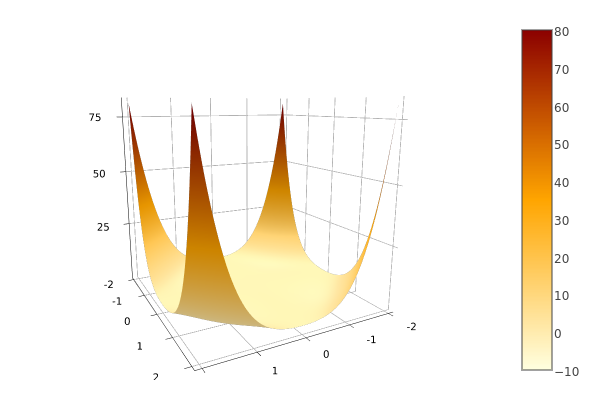
\includegraphics[trim=3cm .7cm 6cm 3cm, clip, width=\textwidth]{motzkin.png}
      \end{column}
    \end{columns}

  \end{frame}
  \begin{frame}{Sum-of-Squares cone}
    \begin{block}{Nonnegative orthant $\R^n_+ \subset \R^n$}
      Proper and self-dual with scalar product
      \[ \la a, b \ra = b^\Tr a. \]
    \end{block}
    \vspace{-1.5em}
    \begin{block}{Semidefinite cone $\Psd \subset \SymK$}
      Proper and self-dual with scalar product
      \[ \la A, B \ra = \trace(B A). \]
    \end{block}
    \vspace{-1.5em}
    \begin{block}{Sum-of-Squares cone $\Sos[n, 2d] \subset \R[x]_{n, 2d}$}
      Proper and dual %$\Sos[2, 2d]^*$
      with scalar product
      \[ \la \mu, p \ra = \int_{\R^n} p(x) \mu(\dif x). \]
      is the cone of \emph{pseudo measures}.
    \end{block}
  \end{frame}
  \begin{frame}{What is Sum-of-squares programming ?}
    %Sum-of-squares programming is a generalization of Semidefinite programming:
    \begin{block}{Linear Programming}
      \vspace{-1em}
      \begin{align*}
        \mini_{x \in \R^n}\quad & \la c, x \ra & \maxi_{y \in \R^n} \quad & \la b, y \ra\\
        \subtoq & Ax = b & \subtoq & A^\Tr y \leq c\\
        & x \geq 0
      \end{align*}
    \end{block}
    \vspace{-2em}
    \begin{block}{Semidefinite Programming}
      \vspace{-1em}
      \begin{align*}
        \mini_{Q \in \SymK} \quad & \la C, Q \ra & \maxi_{y \in \R^n} \quad & \la b, y \ra\\
        \subtoq & \la A_i, Q \ra = b_i & \subtoq & \sum_i A_i y_i \preceq C\\
          & Q \succeq 0
      \end{align*}
      %Linear Programming :
      $A_i = \Diag(a_i), C = \Diag(c), Q = \Diag(x)$
    \end{block}
  \end{frame}
  \begin{frame}{What is Sum-of-squares programming ?}
    \begin{block}{Semidefinite Programming}
      \vspace{-1em}
      \begin{align*}
        \mini_{Q \in \SymK} \quad & \la C, Q \ra & \maxi_{y \in \R^n} \quad & \la b, y \ra\\
        \subtoq & \la A_i, Q \ra = b_i & \subtoq & \sum_i A_i y_i \preceq C\\
          & Q \succeq 0
      \end{align*}
    \end{block}
    \vspace{-2em}
    \begin{block}{Sum-of-squares Programming}
      \vspace{-1em}
      \begin{align*}
        \mini_{p \in \R[x]_{n, 2d}}\quad & \la \nu, p \ra & \maxi\quad \la b, y \ra\\
        \subtoq & \la \mu_i, p \ra = b_i & \subtoq & \sum_i \mu_i y_i \preceq \nu\\
        & p \succeq 0
      \end{align*}
    \end{block}
    \vspace{-1em}
    %Semidefinite Programming:\\
    $(A_k)_{ij} = \la \mu_k, x_ix_j \ra, C_{ij} = \la \nu, x_ix_j \ra, p(x) = x^\Tr Q x$
  \end{frame}
  \begin{frame}{Sum of Squares in Julia : A joint effort}
    \begin{center}
      \scriptsize
      \begin{tikzpicture}
        \SetVertexNormal[Shape=rectangle,FillColor = yellow!50]
        \draw[rounded corners=6pt] (-6.4, 2.5) rectangle (4, 3.5);
        \Vertex[x=-4,y=3,L={\jlpkg{SumOfSquaresOptimization}}]{SOSO}
        \Vertex[x= 0,y=3,L={\jlpkg{SumOfSquares}}]{SOSold}
        \Vertex[x= 3,y=3,L={\jlpkg{MayDay}}]{MD}

        %\draw[->, bend left=20] (-4, 2.5) to (-1, 0.5);
        %\draw[->, bend left=20] (-4, 2.5) to (-1, 0.5);
        \draw[->] (-4, 2.5) .. controls (-1, 2) and (-1, 1.5) .. (-1, 0.5);
        \draw[->] ( 3, 2.5) .. controls (-1, 2) and (-1, 1.5) .. (-1, 0.5);
        \draw[->] ( 0, 2.5) .. controls (-1, 2) and (-1, 1.5) .. (-1, 0.5);

        \draw[rounded corners=6pt] (-6.6, -1.5) rectangle (4, 0.5);
        \Vertex[x=0,y=0,L={\jlpkg{SumOfSquares}}]{SOS}
        \SetVertexNormal[Shape=rectangle,FillColor = blue!30]
        \Vertex[x=3,y=0,L={\jlpkg{PolyJuMP}}]{PJMP}
        \SetVertexNormal[Shape=rectangle,FillColor = green!50]
        \Vertex[x=-4,y=0,L={\jlpkg{MultivariatePolynomials}}]{MP}
        \Vertex[x=-5,y=-1,L={\jlpkg{TypedPolynomials}}]{TP}
        \Vertex[x=-1.5,y=-1,L={\jlpkg{DynamicPolynomials}}]{DP}
        %\tikzset{EdgeStyle/.style={->}}
        \Edge(MP)(TP)
        \Edge(MP)(DP)
      \end{tikzpicture}
    \end{center}
  \end{frame}
  \begin{frame}[fragile]
    \frametitle{Multivariate Polynomial}
    Choose \verb|TypedPolynomials| or \verb|DynamicPolynomials|:
\begin{minted}{Julia}
using TypedPolynomials
@polyvar y # variable with name y
@polyvar x[1:2] # tuple of variables with names x1, x2
\end{minted}
    Build a polynomial from scratch:
\begin{minted}{Julia}
motzkin = x^4*y^2 + x^2*y^4 + 1 - 3x^2*y^2
\end{minted}
    Build a vector of monomials:
\begin{minted}{Julia}
monomials(x, 2) # -> [x1^2, x1*x2, x2^2]
monomials(x, 0:2) # -> [x1^2, x1*x2, x2^2, x1, x2, 1]
\end{minted}
  \end{frame}
  \begin{frame}[fragile]
    \frametitle{PolyJuMP}
    \begin{block}{Constraint}
\begin{minted}{Julia}
m = Model()
@variable m a
@constraint a * x^2 - 2x*y + a * y^2 >= 0
\end{minted}
    \end{block}
      \vspace{-1em}
    \begin{columns}
      \begin{column}{0.6\textwidth}
    \begin{block}{Variable}
      \vspace{-.5em}
\begin{minted}{Julia}
m = Model()
X = monomials([x, y], 0:2)
@variable m p Poly(X)
# p should be strictly positive
@constraint m p >= 1
@constraint m p * motzkin >= 0
solve(m)
\end{minted}
      \vspace{-.5em}
    finds $p(x) = 0.9x^2 + 0.9y^2 + 2$.
    \end{block}
      \end{column}
      \begin{column}{0.4\textwidth}
        \centering
        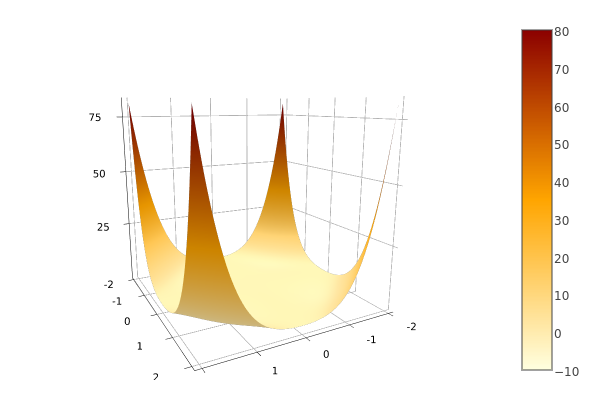
\includegraphics[trim=3cm .7cm 6cm 3cm, clip, width=\textwidth]{motzkin.png}
      \end{column}
    \end{columns}
  \end{frame}
  \begin{frame}[fragile]
    \frametitle{A module and and a solver}
    \begin{block}{Module}
    PolyJuMP needs a polymodule:
\begin{minted}{Julia}
m = Model()
setpolymodule!(m, SumOfSquares)
\end{minted}
    \alert{equivalent} shortcut:
\begin{minted}{Julia}
m = SOSModel()
\end{minted}
    2 lines version useful if \alert{multiple} JuMP extensions used !
    \end{block}
    \begin{block}{Solver}
      SOS variables/constraints need \alert{SDP} solver, e.g. Mosek, SDPA, CSDP, SCS, ...

      DSOS only need \alert{LP} solver and SDSOS only need \alert{SOCP} solver !
    \end{block}
  \end{frame}
  \begin{frame}[fragile]
    \frametitle{Domain constraint}
    \begin{block}{Algebraic Set}
      Finite intersection of algebraic equalities, e.g.
\begin{minted}{Julia}
@set x^2 == y^3 + z^3 && 2x^2 + 3y*z == x^3z^2
\end{minted}
    \end{block}
    \begin{block}{Basic semialgebraic set}
      Finite intersection of algebraic equalities and inequalities, e.g.
\begin{minted}{Julia}
@set x*z >= y^2 && x + z == 1
\end{minted}
    \end{block}
    \begin{columns}
      \begin{column}{0.5\textwidth}
\begin{minted}{Julia}
S = @set x^2 + y^2 == 1
@constraint(m, x^2 + y <= 10,
            domain = S)
\end{minted}
    finds $(3-y/6)^2 + 35/36y^2$.
      \end{column}
      \begin{column}{0.5\textwidth}
        \centering
        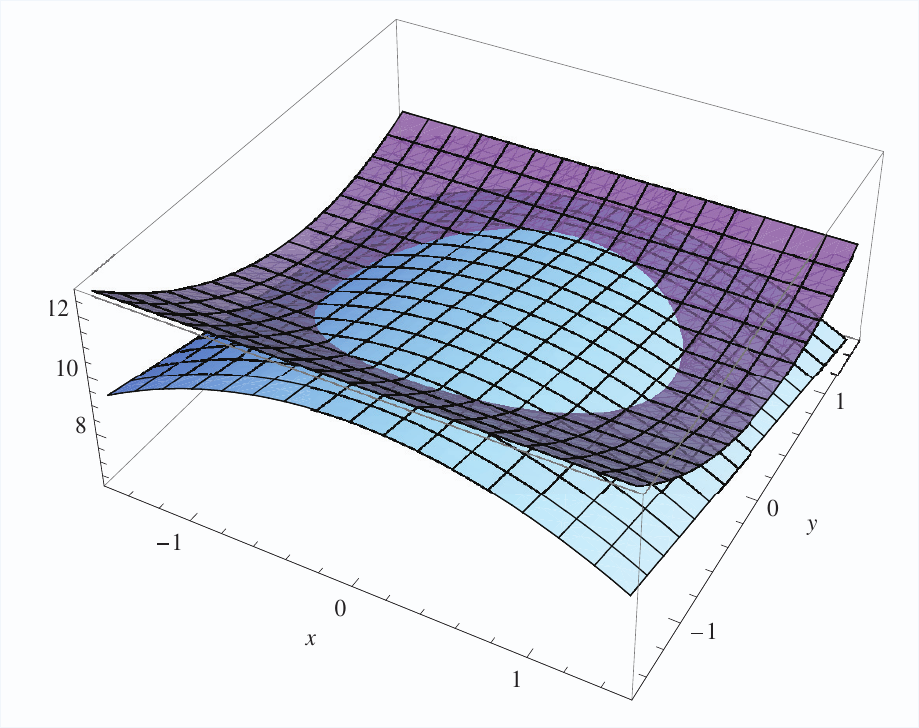
\includegraphics[width=0.7\textwidth]{algebraic_set.png}

        \tiny
        Figure~3.9 of Blekherman, Parrilo and Thomas, 2013, Semidefinite Optimization and Convex Algebraic Geometry.
      \end{column}
    \end{columns}
  \end{frame}
  \begin{frame}[fragile]
    \frametitle{SOS (resp. DSOS and SDSOS)}
    \begin{block}{Variable}
      \vspace{-.5em}
\begin{minted}{Julia}
X = monomials([x, y], 0:2)
@variable m p Poly(X)
\end{minted}
      \vspace{-.5em}
      Variable $p(x) = X^\Tr Q X$ where $Q$ is semidefinite (resp. diagonally dominant, scaled diagonaly dominant).
      \vspace{-.5em}
\begin{minted}{Julia}
@variable m p SOSPoly(X)
@variable m p DSOSPoly(X)
@variable m p SDSOSPoly(X)
\end{minted}
    \end{block}
    \begin{block}{Constraint}
      \vspace{-.5em}
\begin{minted}{Julia}
@constraint m p in SOSCone() # equivalent to p >= 0
@constraint m p in DSOSCone()
@constraint m p in SDSOSCone()
\end{minted}
    \end{block}
  \end{frame}
  \begin{frame}[fragile]
    \frametitle{SOS matrix and SOS convex polynomial}
    \begin{block}{Sum of square matrix}
      \begin{align*}
        P(x) = \begin{bmatrix}x^2 - 2x + 2 & x\\ x & x^2\end{bmatrix} & = \begin{bmatrix}1 & x\\x-1 & 0\end{bmatrix}^\Tr \begin{bmatrix}1 & x\\x-1 & 0\end{bmatrix}\\
        y^\Tr P(x) y & = (y_1 + xy_2)^2 + (x-1)^2y_1^2
      \end{align*}
\begin{minted}{Julia}
@SDconstraint m [x^2-2x+2 x; x x^2] >= 0
\end{minted}
    \end{block}
    \begin{block}{Convex polynomial}
      Positive semidefinite hessian:
      %PolyJuMP:
\begin{minted}{Julia}
@SDconstraint m differentiate(p, x, 2) >= 0
\end{minted}
      %SumOfSquares shortcuts \verb|SOSConvexCone|, \verb|DSOSConvexCone|, \verb|SDSOSConvexCone|.
    \end{block}
  \end{frame}
  \begin{frame}[fragile]
    \frametitle{Newton Polytope}
    \begin{columns}
      \begin{column}{0.6\textwidth}
        \[ p(x) = X^\Tr Q X \qquad X = \ ? \]
        Default : cheap outer approx. $\tilde{\mathcal{N}}(p)$.
        \begin{block}{Exact newton polytope}
\begin{minted}{Julia}
@constraint(m, p >= 0,
newtonpolytope=CDDLibrary(:float))
@constraint(m, p >= 0,
newtonpolytope=CDDLibrary(:exact))
\end{minted}
        \end{block}
        \vspace{-1em}
        \begin{block}{Sparse multipartite}
        \vspace{-1em}
\begin{minted}{Julia}
H = differentiate(p, x, 2)
@constraint(m, y^T H y >= 0,
newtonpolytope=
  (x=>CDDLibrary(:float),
   y=>CheapOuterLibrary()))
\end{minted}
        \end{block}
      \end{column}
      \begin{column}{0.4\textwidth}
        \begin{multline*}
          p(x) = x^4 + 5x^2y^2 - 2x^2y\\- xy^2 + x^2
        \end{multline*}
        \centering
        \tiny
        \begin{tikzpicture}
          \node at (0, 0) {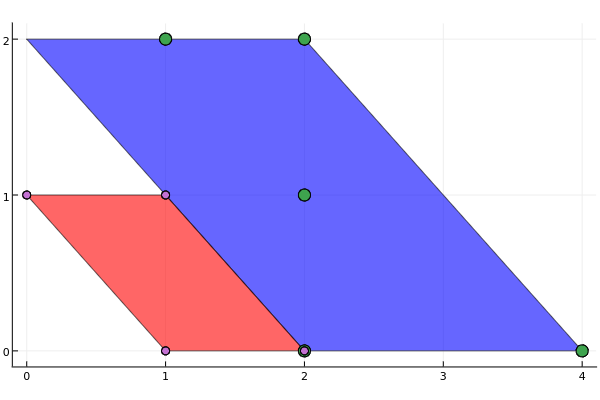
\includegraphics[width=\textwidth]{newton_rough.png}};
          \node at (0, 0.5) {$\tilde{\mathcal{N}}(p)$};
          \node at (-.81, -.6) {$\frac{1}{2}\tilde{\mathcal{N}}(p)$};
        \end{tikzpicture}
        \begin{tikzpicture}
          \node at (0, 0) {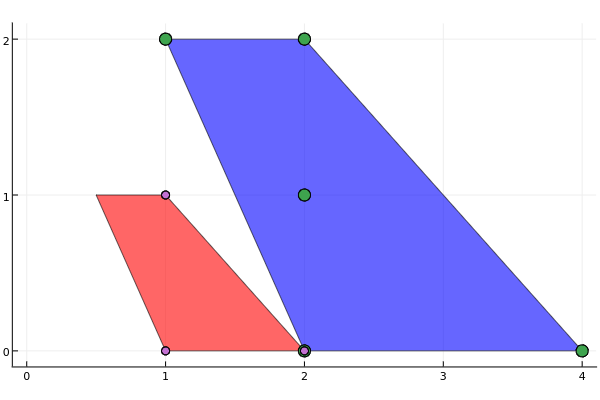
\includegraphics[width=\textwidth]{newton_exact.png}};
          \node at (0, 0.5) {$\mathcal{N}(p)$};
          \node at (-.81, -.6) {$\frac{1}{2}\mathcal{N}(p)$};
        \end{tikzpicture}
      \end{column}
    \end{columns}
  \end{frame}
  \begin{frame}[fragile]
    \frametitle{Application : Polynomial optimization}
      Find $\min_{x \in S} p(x)$, e.g.
\begin{minted}{Julia}
p = x^3 - x^2 + 2x*y - y^2 + y^3
S = @set x >= 0 && y >= 0 && x + y >= 1
\end{minted}
% See Lassere's book pp. 30-31
      SOS program:
\begin{minted}{Julia}
m = SOSModel()
@variable m lb
@objective m Max lb
constr = @constraint m p >= lb, domain = S
\end{minted}
      How to recover the minimizer ?
      Get the dual $\mu$ and check whether it is atomic, i.e.
      \( \mu = \sum_i \lambda_i \delta_{x_i} \).
\begin{minted}{Julia}
AtomicMeasure(getdual(constr))
\end{minted}
      Atomic $\Rightarrow$ $x_i$ global minimizers and \verb|lb| exact minimum.
  \end{frame}
  \begin{frame}[fragile]
    \frametitle{Application : Stability of Switched Systems}
      System $x_{k+1} = A_1x_k$ or $x_{k+1} = A_2x_k$.
      Find a common Lyapunov $V(x)$ such that $V(x) > 0$, $V(A_1x) \leq V(x)$ and $V(A_2x) \leq V(x)$.
\begin{minted}{Julia}
m = SOSModel()
X = monomials(x, 2*d)
@variable m V Poly(X)
@constraint m V >= sum(x.^(2d))
@constraint m constr[i=1:2] V(x=>A[i]*x) <= V
\end{minted}
      How to recover an unstability certificate if it is infeasible ?
\begin{minted}{Julia}
AtomicMeasure.(getdual(constr))
\end{minted}
      Atomic $\Rightarrow$ $\mu_i$ occupation measure of unstable trajectory\footnote{See \jlpkg{SwitchedSystems}}.
  \end{frame}
  \begin{frame}{Future work}
    \begin{itemize}
      \item Symmetry reduction.
      \item Different polynomial basis (Lagrange, orthogonal, ...)
      \item Specialized method for specific algebraic sets (e.g. hypercube) and sampling algebraic varieties.
      \item Modelisation with measures.
      \item Inclusion of decision variables in semialgebraic sets using moment relaxation.
      \item Non-commutative (done), hermitian, orthogonal, idempotent variables.
      \item Syntax for hierarchies.
    \end{itemize}
  \end{frame}
\end{document}
